\documentclass{standalone}
\usepackage{tikz}
\usetikzlibrary{positioning, shapes.geometric}
\usepackage{amsfonts}
\usepackage{amsmath}
\begin{document}

 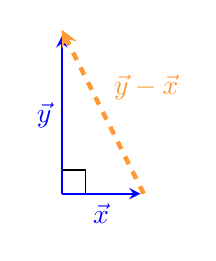
\begin{tikzpicture}[scale=1, every node/.style={scale=1}]
    % Define vectors
    \coordinate (O) at (0,0);
    \coordinate (A) at (0,2);
    \coordinate (B) at (1,0);
    \coordinate (A2) at (0,2.08);
    \coordinate (B2) at (1.04, 0);

    % Draw vectors
    \draw[-stealth, thick, blue] (O) -- (A) node[midway, left] {$\vec{y}$};
    \draw[-stealth, thick, blue] (O) -- (B) node[midway, below] {$\vec{x}$};
    \draw[-stealth, dashed, ultra thick, orange!80] (B2) -- (A2) node[midway, above right] {$\vec{y} - \vec{x}$};

    % Draw right angle symbol
    \draw (0.3,0) -- ++(0,0.3) -- ++(-0.3,0);
\end{tikzpicture}

\end{document}